We value the relationship formed between the client and our team and the importance of having a good relationship. So much so that we want to include you throughout the whole process of building your project by presenting demos and working with your feedback; as well as keeping you up-to-date on our progress.\\

\textbf{Our Methodology}\\
This all forms just one part of the methodology we've chosen to development your project. The agile method. Specifically, feature driven development. One of the biggest advantages about this is that we can quickly and easily incorporate feedback into the system.\\

\textbf{Procedure}\\
We will begin by developing an overall model of the system. The model will represent our solution and how we intend to develop it. Once we have agreed upon the system model we can begin working on the feature list. This list will contain all the features you wish your project to have. We will ranks each as either a major or minor feature and begin working through such accordingly. For each feature we intend to develop a plan to construct the feature.\\

\textbf{Development}\\ 
Lastly, develop the features. As we go through we'll go through each feature on the feature list we'll create the plan, develop the feature and move to the next feature. We believe this will provide the best experience for communication and producing the product.\\
\begin{center}
    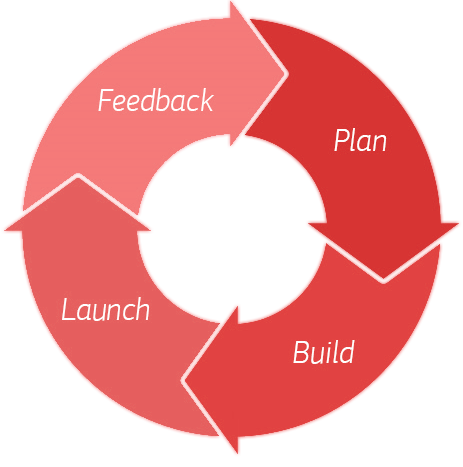
\includegraphics[width=5cm]{../Common/agile.png}
\end{center}
\newpage
\section{Timeline}
\begin{center}
    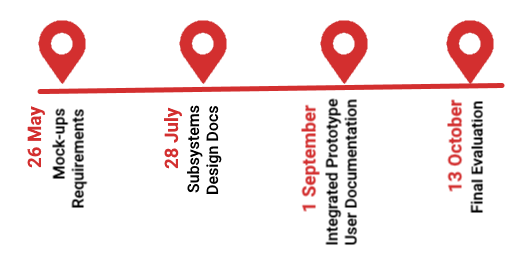
\includegraphics[width=9cm]{../Common/timeline.png}
\end{center}
We would like to meet our clients as soon as possible to begin discussing your vision for the project and to clarify as much as possible
before we begin work. Currently there are 3 demos assigned for this project:
	\begin{itemize}
        \item Demo 1: 26th May
        \item Demo 2: 28th July
        \item Demo 3: 1st September
    \end{itemize}
During these demos we will show you the progress we have made and get feedback from you about what you like and what you would want changed.
Our current plan for the demo meetings are as follows:
	\begin{itemize}
        \item Demo 1: Discuss requirement documentation that we have produced, as well as demo a mock front-end that we have produced to 
        demonstrate how these requirements can be met. 
        \item Demo 2: Discuss design documentation that we have produced, as well as demo the progress we have made with the various subsystems 
        of the project.
        \item Demo 3: Demo the various subsystems of the project, and potentially have a working, integrated prototype of the full system, as 
        well as present some user documentation.
    \end{itemize}
During each of these demo sessions, we would appreciate any feedback that you may have. Any criticisms or advice that you may have for us
will be greatly appreciated, as we greatly value your input and believe that it is important in order to deliver the product that you require.
During the final evaluation phase, which begins on the 13th October, our client will receive all of documentation as well as a fully 
integrated system.\\
\\ 
Please note that, as the client, you are more than welcome to adjust this timetable as you see fit. Additionally if you would like to have any 
additional meetings to check our progress, or make an adjustment to the specification, we would be more than happy to arrange it. We believe 
the more input we get from you as a client, then more refined the final product will be.